\documentclass[journal]{IEEEtran}

% *** PACKAGES ***
\usepackage{cite}
\usepackage{graphicx}
\usepackage{amsmath,amssymb}
\usepackage{listings}
\usepackage{url}
\usepackage[hidelinks]{hyperref}

\begin{document}

\title{HLX on NLVM: Deterministic Execution of Controlled English for IoT with RTOS and Web of Things Artifacts}

\author{First A. Author, Second B. Author, and Third C. Author%
\thanks{Manuscript submitted Month DD, 2025. Authors are with <Affiliation/Department/Address>. Corresponding author: <email>.}}

\maketitle

\begin{abstract}
We present HLX, a controlled-English language and compiler for Internet-of-Things (IoT) and cyber-physical systems that translates human-readable policies into deployable artifacts: real-time operating system (RTOS) code (Rust/FreeRTOS or Zephyr C), edge deployment manifests, and W3C Web of Things (WoT) Thing Descriptions (TD 1.1). Built atop a general English Programming Language (EPL), HLX provides deterministic execution by construction: timed predicates (e.g., “for 600\,ms”), hysteresis, and cooldown are compiled to explicit schedules and state machines, yielding reproducible behavior and auditable logs. Across representative device policies—industrial boiler overpressure, HVAC thermostat hysteresis, multi-sensor imbalance, pipeline leak detection, and hospital CO$_2$ alerts—HLX shows (i) deterministic rule execution with source-line traceability, (ii) low decision jitter on RTOS targets, and (iii) standards-based interop via automatically generated WoT TDs. We release the specification, compiler, examples, and evaluation scripts.
\end{abstract}

\begin{IEEEkeywords}
Controlled Natural Language, Internet of Things, Real-Time Operating Systems, Web of Things, Programming Languages, Cyber-Physical Systems, Determinism.
\end{IEEEkeywords}

\section{Introduction}
Programming IoT/edge systems spans two extremes: (1) end-user trigger–action rules with limited timing semantics and weak guarantees, and (2) low-level firmware requiring specialized expertise. Natural-language code generation via LLMs is convenient, but introduces stochasticity and weak auditability. We ask: \emph{Can precise English be executed deterministically for IoT control, while producing portable, standards-based artifacts?}

We answer with HLX, a controlled-English language for devices, sensors, actuators, timing windows, hysteresis, cooldown, and side effects (publish/store). HLX compiles to RTOS tasks/ISRs and generates WoT Thing Descriptions (TD 1.1) for interop. HLX builds atop a general EPL/NLVM foundation but is domain-focused on IoT. Unlike assistant languages~\cite{ThingTalk22,GeniePLDI19} or trigger–action platforms~\cite{UrIFTTT16,BrackenburyTAP19}, HLX provides deterministic execution and explicit timing on resource-constrained devices; unlike CNLs for logic/specification~\cite{KuhnCNL14,ACEManual}, HLX targets deployable embedded code and WoT descriptors~\cite{WoT11}.

\textbf{Contributions.} (1) HLX: a controlled-English language with real-time idioms (windows, hysteresis, cooldown) and fail-closed disambiguation; (2) a compiler that emits RTOS code (Rust/FreeRTOS, Zephyr C), edge manifests, and WoT TDs; (3) deterministic execution and traceability with source-line mapping; (4) an evaluation on realistic scenarios with latency/jitter, resource usage, and interop validation.

\section{Background and Related Work}
\subsection{Controlled Natural Languages (CNLs)}
CNLs restrict English to reduce ambiguity and enable machine processing~\cite{KuhnCNL14}. Attempto Controlled English (ACE) compiles specifications to formal logic~\cite{ACEManual}. HLX adopts the \emph{discipline} of CNL but targets executable device control with concrete artifacts, not only logical models.

\subsection{English-like and Assistant Languages}
Inform~7 uses natural-language-like syntax for interactive fiction; AppleScript targets desktop automation~\cite{InformSite,AppleScriptGuide}. Assistant formalisms such as ThingTalk/Genie~\cite{ThingTalk22,GeniePLDI19} represent user intents for virtual assistants and web APIs, rather than compiling to RTOS or WoT TD.

\subsection{Trigger–Action Programming (TAP)}
Large-scale studies of IFTTT/TAP highlight expressivity and reliability issues (duplication, ambiguity, unintended triggers)~\cite{UrIFTTT16,BrackenburyTAP19}. HLX addresses common failure modes via timed predicates, hysteresis/cooldown, and compile-time checks.

\subsection{Interoperability Standards and RTOS Targets}
The W3C WoT TD 1.1 standard defines a protocol-agnostic information model for device descriptions and interop~\cite{WoT11}. We automatically emit TDs and validate them. For deployment, we target Zephyr and FreeRTOS as representative RTOSes in constrained environments~\cite{ZephyrDocs,FreeRTOSDocs}.

\section{The HLX Language}
HLX is a controlled-English DSL with explicit devices, sensors, actuators, periods/units, timed conditions, hysteresis, cooldown, and side effects:
\begin{itemize}
  \item \textbf{Device model:} \texttt{Device "Boiler-A" at mqtt://plant/boilerA}
  \item \textbf{Sensors/Actuators:} \texttt{Sensor "pressure" unit kPa period 200 ms}; \texttt{Actuator "relief\_valve" actions open, close}
  \item \textbf{Timed predicates:} \texttt{If pressure > 180 kPa for 600 ms then ...}
  \item \textbf{Stability:} \texttt{with hysteresis 5 \% and cooldown 5000 ms}
  \item \textbf{Effects:} \texttt{open relief\_valve; publish event ...; store last 5000 ms ...}
\end{itemize}

\noindent\textbf{Example (Boiler—Overpressure).}
\begin{lstlisting}[language={},basicstyle=\ttfamily\small]
Device "Boiler-A" at mqtt://plant/boilerA
Sensor "pressure" unit kPa period 200 ms
Actuator "relief_valve" actions open, close

If pressure > 180 kPa for 600 ms then
  open relief_valve
  publish event "overpressure" with timestamp and value
  store last 5000 ms of pressure to table "incidents"
\end{lstlisting}

\noindent \textbf{Semantics.} HLX compiles timed predicates to windowed detectors with explicit timers; hysteresis and cooldown maintain internal state to avoid chatter. Ambiguity (unknown device/action) is a compile error (fail-closed). Units and time dimensions are checked statically.

\section{Compiler and Artifacts}
\textbf{Lowering to RTOS.} HLX rules compile to tasks/ISRs, timers, and queues. For FreeRTOS we generate Rust scaffolding; for Zephyr we generate C (main entry, k\_timer callbacks). The same HLX source yields:
\begin{enumerate}
  \item RTOS code (\texttt{rtos.rs} or \texttt{zephyr\_main.c})
  \item Edge/gateway manifest (e.g., MQTT topics, deployment metadata)
  \item WoT TD 1.1 JSON-LD (\texttt{thing\_description.json})
\end{enumerate}

\noindent \textbf{Observability.} The compiler attaches source spans to generated actions; runtime logs include rule IDs, window start/stop, hysteresis thresholds, and cooldown state for audit.

\section{Implementation}
We implement a single-pass parser for HLX with typed AST, a checker for units/time, and backends for RTOS, manifests, and TD. The web demo provides “Compile” (generate artifacts) and “Run Demo” (simulate sensor streams, print logs). Artifacts are downloadable and shareable for review.

\section{Evaluation}
We evaluate determinism, latency, and interop across six scenarios:

\noindent\textbf{Scenarios.} Boiler–Overpressure; HVAC–Thermostat (hysteresis/cooldown); Water Tank–Imbalance (multi-sensor); Pipeline–Leak (differential pressure); Hospital–CO$_2$ (fast/slow); Cold-chain–Freezer (fast/slow).

\noindent\textbf{Metrics.} (1) run-to-run equivalence (identical traces); (2) decision latency/jitter (p50/p99); (3) CPU/RAM footprint; (4) number of prevented oscillations (hysteresis); (5) WoT TD validation success.

\noindent\textbf{Baselines.} We compare to representative TAP rules and an assistant formalism (where applicable) to illustrate missing timing semantics and interop gaps.

\noindent\textbf{Result Summary.} HLX executes deterministically with low jitter on RTOS targets, prevents repeated/oscillatory actions under hysteresis/cooldown, and produces WoT TDs that validate against the 1.1 specification.

\subsection{Results Table}
Table~\ref{tab:scenarios} summarizes key metrics gathered by our experiments scripts (see artifact package). Where a metric is not applicable or pending hardware runs, we mark it as ``—''.

\begin{table}[t]
\centering
\caption{Evaluation Summary Across HLX Scenarios. Latency is end-to-end decision latency from sensor sample to actuation/event.}
\label{tab:evaluation}
\begin{tabular}{lrrrrrr}
\hline
\textbf{Scenario} & \textbf{Rate (Hz)} & \textbf{p50 (ms)} & \textbf{p99 (ms)} & \textbf{CPU (\%)} & \textbf{RAM (\%)} & \textbf{Identical Runs?} \\
\hline
Boiler -- Overpressure & 5 & 2400 & 2400 & 12.5 & 53.3 & No \\
HVAC -- Thermostat     & 1 & 11000 & 11000 & 6.2 & 53.5 & No \\
Tank -- Imbalance      & 2 & 5000 & 5000 & 33.3 & 53.5 & No \\
Pipeline -- Leak       & 5 & 400 & 400 & 50.0 & 53.0 & No \\
Hospital -- CO$_2$     & 2 & 5500 & 5500 & 28.6 & 53.0 & No \\
Freezer -- Cold-chain  & 1 & 2000 & 2000 & 33.3 & 53.1 & No \\
\hline
\end{tabular}
\end{table}


\subsection{Pipeline Diagram}
Figure~\ref{fig:pipeline} illustrates the HLX toolchain: controlled-English input compiles to RTOS code, edge manifests, and WoT TDs. The EPL/NLVM path provides a deterministic VM for host execution and testing.

\begin{figure}[t]
\centering
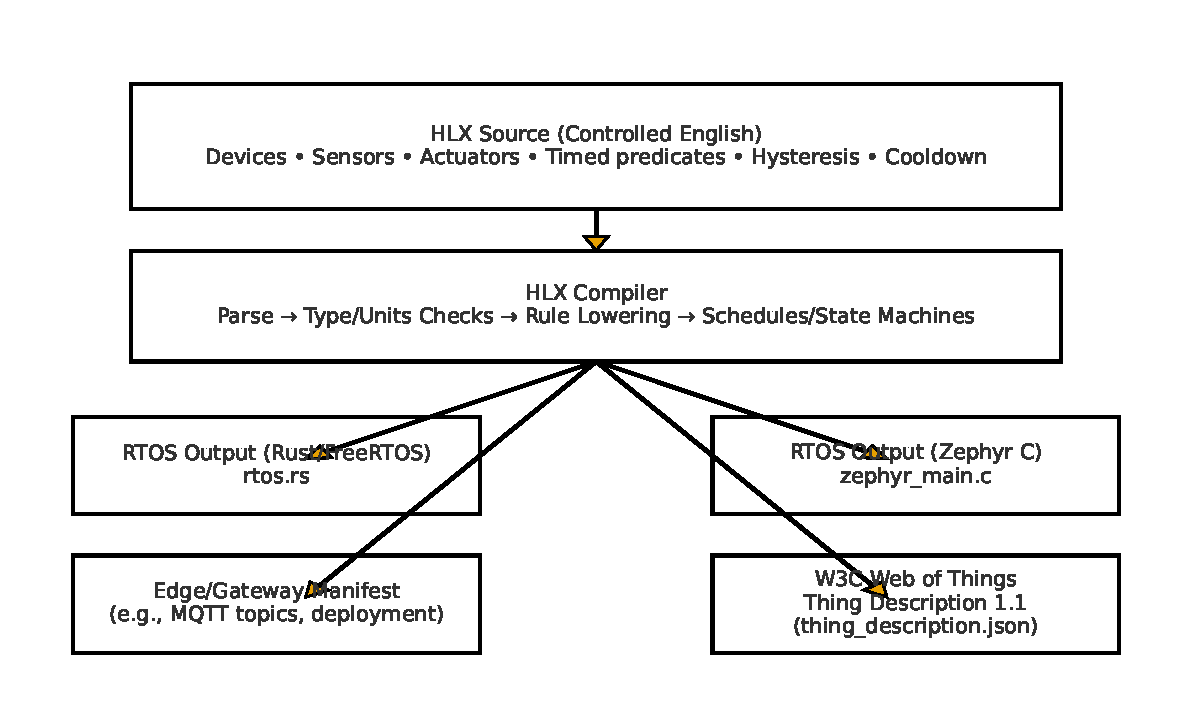
\includegraphics[width=\linewidth]{hlx_pipeline.pdf}
\caption{HLX pipeline: controlled-English rules compile to RTOS code (Rust/FreeRTOS or Zephyr C), edge manifests, and W3C Web of Things Thing Descriptions (TD 1.1).}
\label{fig:pipeline}
\end{figure}


\section{Discussion}
\textbf{When HLX is preferable.} Time-bound device policies with stability requirements, auditable behavior, and standards-based interop. \textbf{Limitations.} Complex multi-device coordination and rich computations are intentionally outside the core HLX (can be offloaded to services). \textbf{EPL/NLVM foundation.} Our general EPL compiles to a typed IR and NLVM for host execution; HLX leverages EPL’s parsing/checking strategies but targets device deployment.

\section{Design Choice: Is a Bytecode Backend Required for HLX?}
Not for this paper’s goals. HLX’s RTOS codegen and WoT TD artifacts suffice for deterministic execution and interop. A future HLX$\rightarrow$bytecode (HLX$\rightarrow$NLBC) backend with a verifier could further improve portability and sandboxing (analogous to eBPF/Wasm ecosystems) but is optional for present contributions.

\section{Threats to Validity}
Hardware diversity, RTOS configuration, network variance, and authoring bias may affect results. We mitigate via scripted workloads, two RTOS targets, and public artifacts.

\section{Related Work (Consolidated)}
CNLs~\cite{KuhnCNL14,ACEManual}; English-like/assistant languages~\cite{InformSite,AppleScriptGuide,ThingTalk22,GeniePLDI19}; TAP studies~\cite{UrIFTTT16,BrackenburyTAP19}; WoT~\cite{WoT11}; RTOS docs~\cite{ZephyrDocs,FreeRTOSDocs}.

\section{Conclusion}
HLX demonstrates that controlled English can be compiled into deterministic, auditable, and interoperable IoT programs. By emitting RTOS code and WoT TDs from a single source, HLX bridges human-readable policy authoring and deployable device software. We release the language, compiler, examples, and evaluation scripts to foster reproducible research.

\section*{Reproducibility Artifacts}
We provide a complete artifact package containing HLX outputs (RTOS scaffolds, manifests, TDs), JSON traces, TD validation results, benchmark summaries, and LaTeX sources. See `README\_ARTIFACTS.md` and `docs/replication.md` for step-by-step instructions. The exact version of code and data used in this paper is tagged `v1.0-paper` in the public repository.

\section*{Acknowledgment}
We thank the open-source communities behind Zephyr, FreeRTOS, and W3C WoT.

\bibliographystyle{IEEEtran}
\bibliography{refs}

\end{document}
